% Artículo del Proyecto Grupal 1. Formato IEEE, máximo 4 páginas con referencias.
\documentclass[conference]{IEEEtran}
\usepackage[spanish,es-noshorthands,es-tabla]{babel}
\usepackage[utf8]{inputenc}
\usepackage[T1]{fontenc}
\usepackage{amsmath,amssymb}
\usepackage{graphicx}
\usepackage{booktabs}
\usepackage{xcolor}
\usepackage{cite}
\usepackage{url}
\usepackage{float}
\usepackage[hidelinks]{hyperref}
\newcommand{\repo}{https://github.com/TamaraCM06/tcajiao_asm_2026_s2/blob/master/proyecto_1_grupal}
\usepackage{tikz}
\usetikzlibrary{positioning,arrows.meta,fit}
\graphicspath{{figuras/}}

\begin{document}

\title{Sistema distribuido de reducción adaptativa de ruido con filtrado FIR y espectral sobre microcontroladores}

\author{\IEEEauthorblockN{Nicolás Florez Jiménez, Tamara Vanessa Cajiao Molina, Santiago Robles Obando, Santiago Boza Quiros}
\IEEEauthorblockA{Escuela de Ingeniería en Computadores, Instituto Tecnológico de Costa Rica, Cartago, Costa Rica\\
CE 1110 Análisis de Señales Mixtas, II Semestre 2026}}

\maketitle

\begin{abstract}
This paper presents a three-node wired system that acquires a noisy signal,
characterizes its noise and reduces it in quasi real time with two independent
strategies. An RP2040 acquisition node samples the input at 16~kHz with DMA, removes
the DC component, applies a Hann window and a 256-point FFT for diagnosis, and streams
256-sample blocks to an ESP32 through SPI frames with a sequence identifier and a
CRC-8 checksum. The ESP32 runs two independent processing
paths: a 75-tap Kaiser FIR low-pass filter with linear phase and a block spectral
method based on a 1024-point radix-2 FFT, 50\,\% overlap-add and an adaptive relative
threshold that preserves conjugate symmetry. The output is played through an 8-bit DAC
followed by a second-order Sallen-Key reconstruction filter; a host computer only
stores data, tunes parameters and relays playback. A Python model with a direct DFT
and FIR and IIR candidates guided the design. Quality metrics are computed on the ESP32
over controlled signals with a clean reference, and its outputs agree with
Python by more than 99.99\,\%; microphone captures validate the physical chain by
listening and spectra. On the board, with noise outside the useful band
the FIR filter improved the SNR by 58--60~dB and the spectral method by 18--20~dB;
with white noise both gained about 6~dB, using about 9~ms of processing per 16~ms
block. When noise overlaps the useful band neither method improves the SNR without
removing useful energy, quantifying the noise--distortion trade-off.
\end{abstract}

\begin{IEEEkeywords}
noise reduction, FIR filter, spectral filtering, FFT, embedded systems, distributed acquisition
\end{IEEEkeywords}

\section{Introducción}
Toda señal adquirida desde un sensor llega acompañada de interferencias: tonos de
equipos cercanos, ruido de banda ancha del propio circuito o perturbaciones
impulsivas. Reducirlas en el mismo sistema embebido que adquiere la señal, sin
depender de una computadora, exige elegir con cuidado la frecuencia de muestreo, el
tamaño de bloque, el formato numérico y el método de filtrado, porque memoria, tiempo
de cálculo y ancho de banda del enlace son limitados~\cite{enunciado}.

Este trabajo diseña, implementa y evalúa un sistema de tres nodos cableados: un nodo de
adquisición y análisis en una Raspberry Pi Pico y dos rutas de procesamiento
independientes en una ESP32, una temporal (FIR) y otra espectral (FFT/IFFT) con
cálculo de métricas. Ambos métodos se diseñaron primero en un modelo de Python que
también sirve de referencia para validar el firmware.

La Sección~\ref{sec:teoria} resume los fundamentos teóricos. La
Sección~\ref{sec:diseno} describe la arquitectura, el enlace entre nodos y el diseño de
ambos filtros. La Sección~\ref{sec:resultados} presenta y analiza los resultados, y las
Secciones~\ref{sec:conclusiones} y~\ref{sec:recomendaciones} cierran con conclusiones y
recomendaciones.

\section{Marco teórico}\label{sec:teoria}
\textbf{Convolución y respuesta en frecuencia.} Un sistema lineal e invariante en el
tiempo responde con $y[n]=x[n]*h[n]$, que en frecuencia equivale a
$Y(e^{j\omega})=X(e^{j\omega})H(e^{j\omega})$~\cite{oppenheim2010}. La respuesta
$H(e^{j\omega})=|H(e^{j\omega})|e^{j\angle H(e^{j\omega})}$ es compleja: la magnitud
fija la atenuación de cada frecuencia y la fase su retardo.

\textbf{FIR, IIR y transformada Z.} La ecuación de diferencias
\begin{equation}
y[n]=\sum_{k=0}^{M} b_k x[n-k]-\sum_{k=1}^{N} a_k y[n-k]
\end{equation}
tiene función de transferencia $H(z)=\sum b_k z^{-k}/(1+\sum a_k z^{-k})$. Un sistema
causal es estable si todos sus polos están dentro del círculo unitario, con región de
convergencia $|z|>\max_k|p_k|$. Un FIR ($a_k=0$) solo tiene polos en $z=0$, es siempre
estable y, con coeficientes simétricos, tiene fase lineal y retardo constante de $M/2$
muestras~\cite{proakis2007}.

\textbf{DFT, FFT y ventanas.} La DFT de $N$ muestras,
$X[k]=\sum_{n=0}^{N-1}x[n]e^{-j2\pi kn/N}$, cuesta $O(N^2)$; la FFT radix-2 la calcula en
$O(N\log_2N)$ si $N=2^m$~\cite{cooley1965}. La resolución es $\Delta f=f_s/N$. Truncar
un bloque produce fuga espectral; la ventana Hann reduce los lóbulos laterales a cambio
de un lóbulo principal más ancho~\cite{harris1978}. Al usar Hann simétrica en análisis
y síntesis, la superposición se normaliza por la suma de sus cuadrados para
reconstruir~\cite{allen1977}. Para que la IFFT de un espectro modificado sea real se debe
conservar $X[N-k]=X^*[k]$.

\textbf{Métricas.} Con referencia limpia $s[n]$ y salida alineada $\hat s[n]$ sobre $L$
muestras:
\begin{equation}
\mathrm{MSE}=\tfrac{1}{L}\textstyle\sum(s-\hat s)^2,\quad
\mathrm{SNR_{dB}}=10\log_{10}\dfrac{\sum s^2}{\sum (s-\hat s)^2},
\end{equation}
y $E_x=\sum|x[n]|^2$. La mejora es $\Delta\mathrm{SNR}=\mathrm{SNR}_{out}-\mathrm{SNR}_{in}$.
La energía útil conservada es $100\,E_{\tilde s}/E_s$, con $\tilde s$ la referencia
procesada por el mismo filtro, y la atenuación compara la energía del ruido de entrada
con la del residuo $\hat s-\tilde s$.

\section{Diseño e implementación}\label{sec:diseno}

\subsection{Arquitectura y flujo de datos}
La Fig.~\ref{fig:sistema} (Anexo~\ref{sec:anexo}) muestra el sistema. El nodo~1 (RP2040) muestrea la entrada
por su ADC de 12~bits a $f_s=16$~kHz con DMA, en bloques de $N=256$ (16~ms,
$\Delta f=62.5$~Hz)~\cite{rp2040}. Elimina la media de cada bloque y, sobre una copia,
aplica Hann y FFT para estimar el nivel, la frecuencia dominante y la saturación. Las
muestras sin componente DC se envían a la ESP32, donde dos rutas con estado
independiente ejecutan el FIR (nodo~2) y el método espectral (nodo~3), permitido por
el enunciado al ser un microcontrolador de doble núcleo~\cite{enunciado,esp32ds}. La
computadora solo almacena, ajusta parámetros y solicita la reproducción; no filtra. La
terminal de la PC funciona como interfaz local del nodo~3: muestra el método activo, la
energía conservada, el MSE y la SNR antes y después que calcula la ESP32.


\textbf{Enlace entre nodos.} Cada bloque viaja por SPI a 2~MHz en una trama de
1032~bytes: cabecera (2), identificador de secuencia (4), 256 muestras en float32 (1024),
CRC-8 con polinomio $x^8+x^2+x+1$ (1) y un byte de relleno~\cite{peterson1961}. La
ESP32, esclava SPI~\cite{espidf}, controla el flujo con una línea READY y rechaza tramas
con longitud, cabecera o CRC inválidos o con muestras no finitas; el identificador
revela saltos, duplicados y retrocesos. Cualquier pérdida o cola llena aborta la
captura y queda registrada. El enlace con la PC usa paquetes PCM16 con índice y CRC-32 a
1~Mbaud, tras fallar el diagnóstico del puente USB a una tasa superior.

\textbf{Justificación conjunta.} Los tonos y bandas generados no superan 4~kHz, por lo que
$f_s=16$~kHz deja Nyquist en 8~kHz con margen~\cite{oppenheim2010}. El flujo útil es
$16\,000\times4$~B $=64$~kB/s, holgado frente a los 250~kB/s del SPI a 2~MHz. Hacia la
PC viajan tres señales PCM16 (96~kB/s) sobre unos 99~kB/s útiles a 1~Mbaud: una
ocupación cercana al 97\,\%, verificada con una captura completa sin pérdidas. Los bloques de 256 (FIR) y 1024
con salto de 512 (espectral) son potencias de dos~\cite{enunciado}.
Los estímulos se sintetizan a 16~kHz, por lo que su espectro queda acotado por
construcción bajo Nyquist y las pruebas no presentan aliasing; una componente externa
sobre 8~kHz sí se plegaría, pues el Sallen-Key filtra la salida del DAC, no la entrada
del ADC~\cite{oppenheim2010}.

\subsection{Filtro temporal (nodo 2)}
Con banda de paso hasta 1.6~kHz, rechazo desde 2.4~kHz, rizado de 0.1~dB y atenuación
mínima de 60~dB se compararon un FIR por ventana Kaiser~\cite{kaiser1974} y tres IIR
(Tabla~\ref{tab:filtros}). Se eligió el FIR de orden~74: es incondicionalmente estable
(sus 74 polos están en $z=0$, ROC $|z|>0$), tiene fase lineal con retardo constante de
37~muestras (2.3~ms) y obtuvo la mayor SNR. Los IIR requieren menos operaciones, pero
su retardo de grupo varía en la banda útil y deforma los transitorios. Su diagrama de polos y ceros y su respuesta en
frecuencia están en la Fig.~\ref{fig:fir} (Anexo~\ref{sec:anexo}).

\begin{table}[H]
\centering
\caption{Candidatos de filtro temporal (simulación, P2)}
\label{tab:filtros}
\begin{tabular}{lcccc}
\toprule
Filtro & Orden & MAC & Retardo & SNR (dB) \\
\midrule
FIR Kaiser & 74 & 75 & 37 & 65.1 \\
Butterworth & 20 & 50 & 18.4--24.7 & 15.5 \\
Chebyshev I & 10 & 25 & 13.3--20.6 & 14.8 \\
Elíptico & 6 & 15 & 6.0--10.6 & 18.6 \\
\bottomrule
\end{tabular}
\end{table}


En la ESP32 el FIR procesa muestra a muestra con un anillo de 75 posiciones en float32
y coeficientes exportados desde Python, con $H(z)=\sum_{k=0}^{74}b_kz^{-k}$.
La salida se convierte a PCM16 con saturación
explícita y, para la reproducción, a 8~bits del DAC, lo que limita el rango dinámico a
unos 48~dB. En los WAV de la ESP32, un ajuste conjunto de senos y cosenos sobre 93
bloques, excluyendo el arranque, difiere menos de 0.0035~dB de la respuesta calculada
en 440/880/1320~Hz. A 4~kHz solo se resuelve una cota de $-58.4$~dB, frente a
$-73.0$~dB calculados: la cuantización PCM16 limita esta medida digital antes del DAC.

\subsection{Filtro espectral y evaluación (nodo 3)}
El método procesa bloques de $N=1024$ ($\Delta f=15.625$~Hz) con salto de 512:
\begin{enumerate}
\item multiplicar el bloque por Hann;
\item calcular la FFT radix-2~\cite{cooley1965};
\item proteger los bins bajo $f_{min}$ (1.6~kHz);
\item marcar como ruido cada bin no protegido cuya energía $|X[k]|^2$ supere un umbral
relativo (0.05) a la máxima energía de esa región, con piso de 0.001 del pico global,
junto con sus vecinos dentro de un
ancho total de 100~Hz;
\item multiplicar esos bins y sus conjugados por un factor real (0.1);
\item calcular la IFFT, volver a aplicar Hann y reconstruir por superposición y suma
normalizada por $\sum w^2$~\cite{allen1977}.
\end{enumerate}
El umbral se recalcula en cada bloque, por lo que la selección sigue la interferencia
si cambia de frecuencia o de nivel~\cite{boll1979}. Los cuatro parámetros se cambian en
ejecución desde la terminal, sin recompilar. El mismo nodo acumula, en doble precisión,
MSE, SNR de entrada y salida, energía útil conservada, atenuación de la interferencia y
tiempo por bloque.

\subsection{Reconstrucción analógica}
La salida del DAC pasa por un divisor de 10~k$\Omega$/10~k$\Omega$, un seguidor (LM358,
amplificador~A) y un Sallen-Key pasabajos de ganancia unitaria (amplificador~B) con
$R_1=R_2=4.7$~k$\Omega$, $C_1=22$~nF de realimentación y $C_2=10$~nF a
tierra~\cite{sallen1955,sloa024,lm358}, alimentado a 5~V. Su frecuencia de corte
$f_c=1/(2\pi\sqrt{R_1R_2C_1C_2})\approx2283$~Hz y su $Q=\tfrac12\sqrt{C_1/C_2}\approx0.74$
atenúan las imágenes del DAC antes del amplificador. Se usó 22~nF, valor comercial
disponible, en lugar de los 20~nF de un Butterworth exacto ($Q=0.707$, 2394~Hz); el
cambio produce un ligero realce de $+0.3$~\% bajo 1~kHz. Con el sistema en marcha se
midieron 5~V en la alimentación y 0.815~V en la entrada y la salida del seguidor, la
mitad del nivel medio del DAC, como predice el divisor.

Para comparar las amplitudes muestreadas se usa
$|H_{med}(f)|=|H_{SK}(f)|\,|\mathrm{sinc}(f/16000)|$: la retención del DAC atenúa
la fundamental~\cite{dacretencion}. La curva representa esa componente, sin ajustar
los componentes físicos ni modelar imágenes que se pliegan al adquirir a 16~kHz.

\section{Resultados y análisis}\label{sec:resultados}
\textbf{Criterios de aceptación}, fijados antes de las pruebas finales: con ruido fuera
de banda, $\Delta\mathrm{SNR}\geq10$~dB y energía útil conservada $\geq90$\,\%; en todos
los casos, tiempo máximo por bloque menor que su duración (16~ms FIR, 32~ms espectral);
cero pérdidas de bloque. Para el filtro analógico, error de ganancia $\leq15$\,\% por tono
con variabilidad $\leq10$\,\%. La concordancia entre la salida de la placa y el modelo de
Python, $100\max(0,1-\mathrm{RMSE}/\mathrm{RMS})$, debe ser $\geq90$\,\% para ambas
rutas: admite NRMSE hasta 0.1 y comprueba equivalencia, no eliminación de ruido.
El criterio analógico se fijó antes de medir; la corrección física de retención se
documentó después como reanálisis, conservando las medidas y los criterios originales.

\textbf{Protocolo de prueba.} Para las métricas, la PC envía a la ESP32 el CSV de
cada caso con la mezcla y la referencia $s[n]$ del modelo, y la placa filtra y calcula
MSE, SNR, energía útil, atenuación y tiempos. P1 es un tono con interferencia de
4~kHz; P2, tres tonos con ruido de 2.5--3.8~kHz; P3, un barrido con ruido blanco; P4,
transitorios con impulsos; P5, ruido superpuesto de 600--1500~Hz. Para la cadena
física el audio suena frente al micrófono y recorre Pico, SPI y ESP32; sin referencia
alineada no hay métricas de calidad, y se verifican tiempos, pérdidas, espectros y
sonido. Una captura de 6~s entregó 375 bloques a 16\,000.26 muestras/s, sin pérdidas,
errores SPI ni recortes. P6 se ejecuta en la defensa.

\textbf{Resultados en placa.} La Tabla~\ref{tab:pruebas} resume 14 evaluaciones
completas; tres intentos se abortaron al detectar tramas USB truncadas y se repitieron.
Las métricas de calidad no varían entre corridas porque el procesamiento de un mismo
CSV es determinista; la variabilidad aparece en los tiempos (desviación $\leq8~\mu$s).
La salida de la placa coincide con Python sobre el mismo PCM16 con concordancia
$\geq99.999$\,\% en ambas rutas~\cite{numpy2020,scipy2020}.
% Sustituir con estadisticas de sesiones reales de P1--P5; no fabricar filas sin medicion.
\noindent\textit{Pendiente: tabla de P1--P5 con tres repeticiones por condición,
parámetros, media y variabilidad; distinguir evaluación CSV en placa y adquisición ADC.}


\textbf{Comparación de métodos.} Con ruido fuera de banda (P1, P2) ambos cumplen los
criterios: el FIR mejora 58--60~dB y atenúa la interferencia 70--73~dB, porque toda su
banda de rechazo queda bajo $-60$~dB; el espectral mejora 18--20~dB, limitado por el
factor 0.1 ($-20$~dB). Con ruido blanco (P3) ambos ganan cerca de 6~dB: solo se quita el
ruido sobre la banda útil, unas 3/4 partes de su potencia ($10\log_{10}4$). En P4 la
energía de los impulsos cae en la banda útil y la mejora es de 0.1--0.2~dB; su evidencia
es la respuesta temporal. El cálculo medio conjunto fue 8.4--9.5~ms por bloque de
16~ms, con 2.5~ms por bloque FIR y 3.7~ms por ventana espectral, incluida la ruta de
referencia; el máximo conjunto, 25.9--31.5~ms, queda bajo el salto de 32~ms. El estado
DSP ocupa 102\,080~B y quedaron libres al menos 67~kB de memoria. La latencia
algorítmica del FIR es 2.3~ms más el bloque de 16~ms; la del espectral, una ventana de
64~ms más 2.3~ms de alineación. Al evaluar CSV el enlace USB transporta entrada,
referencia y salidas, por lo que 6~s de señal tardan unos 16~s y la latencia digital
medida (116~ms) no representa la captura en tiempo real.

\textbf{Compromiso ruido--distorsión.} En P5 el ruido comparte la banda útil y
ninguno de los dos métodos mejora la SNR, porque proteger la señal útil también protege
el ruido superpuesto. Al bajar $f_{min}$ a 600~Hz, el espectral mejora 5.9~dB con factor
0.1 pero conserva solo 72\,\% de la energía útil, frente a 1.8~dB y 90\,\% con factor 0.8
(Fig.~\ref{fig:compromiso}, Anexo~\ref{sec:anexo}).


\textbf{Comparación analógica.} La captura del 5/11 a las 18:57 UTC cumple en los tres
tonos útiles (Tabla~\ref{tab:analogica}). A 4~kHz la amplitud varía 19.3\,\%, por encima
del 10\,\% fijado: ese punto no permite validar el criterio. La imagen del
DAC en 12~kHz se pliega sobre 4~kHz al adquirir a 16~kHz; el modelo nominal estima una
contribución cercana al 4\,\% de la fundamental filtrada. Es una limitación posible,
sin atribuirle todo el error observado ni relajar los criterios.
\begin{table}[H]\centering\footnotesize
\caption{Ganancia analógica medida frente a Sallen-Key con retención DAC.}
\label{tab:analogica}
\begin{tabular}{rrrrl}\toprule
Hz & Modelo & Medida & Error (\%) & Estado \\\midrule
440 & 0.5007 & 0.4881 & 2.52 & Cumple \\
880 & 0.4987 & 0.4958 & 0.59 & Cumple \\
1320 & 0.4823 & 0.4343 & 9.95 & Cumple \\
4000 & 0.1433 & 0.0972 & -- & Inválida \\\bottomrule
\end{tabular}\end{table}

\section{Conclusiones}\label{sec:conclusiones}
La arquitectura implementada mantiene la adquisición separada en
la Pico y la ESP32 ejecuta dos rutas de filtrado independientes dentro de su
presupuesto de tiempo, con un enlace que delimita bloques, detecta errores y reporta
pérdidas, verificado con una captura física completa. La coincidencia entre el modelo de Python y el firmware muestra que el diseño
validado en simulación se trasladó al microcontrolador sin cambiar su comportamiento.
Cuando el ruido está separado en frecuencia, el FIR ofrece la mayor reducción con fase
lineal y menor latencia, mientras que el método espectral reduce menos pero se adapta
por bloque a interferencias cambiantes sin rediseñar coeficientes. Cuando ruido y señal
comparten frecuencias, ningún filtro lineal ni ganancia espectral puede separarlos sin
quitar información útil, y la elección de parámetros pasa a ser una decisión de
compromiso entre ruido residual y distorsión.

\section{Recomendaciones}\label{sec:recomendaciones}
Se recomienda colocar un filtro antialias analógico antes del ADC de la Pico y medir su
respuesta, ya que la protección contra aliasing hoy depende del contenido de la señal.
Un DAC externo de mayor resolución o una salida PWM de alta frecuencia mejoraría el
rango dinámico de la reproducción, limitado por los 8~bits del DAC interno. En el
método espectral convendría estimar el piso de ruido durante silencios y aplicar
sustracción espectral con un suelo mínimo de ganancia, para mejorar el caso de ruido
superpuesto sin introducir ruido musical. Finalmente, ejecutar cada ruta en un núcleo
distinto de la ESP32 permitiría reducir la latencia de extremo a extremo.

\bibliographystyle{IEEEtran}
\bibliography{referencias}

\appendices
\section{Figuras complementarias}\label{sec:anexo}
\begin{figure}[H]
\centering
\begin{tikzpicture}[font=\footnotesize, node distance=5mm and 5mm,
  b/.style={draw, rounded corners=2pt, align=center, minimum height=10mm, minimum width=17mm, inner sep=2pt},
  a/.style={-{Latex[length=2mm]}, thick}, l/.style={font=\footnotesize, fill=white, inner sep=1pt}]
\node[b] (pico) {Nodo 1: Pico\\ADC 16 kHz, DC\\Hann+FFT (diagnóstico)};
\node[b, left=7mm of pico] (mic) {Micrófono\\MAX4466};
\node[b, below=12mm of pico, xshift=-17mm] (fir) {Nodo 2\\FIR 75 coef.};
\node[b, below=12mm of pico, xshift=17mm] (esp) {Nodo 3\\FFT/IFFT\\y métricas};
\node[b, below=34mm of pico] (pc) {PC: WAV y\\parámetros};
\node[b, below=11mm of pc, xshift=-22mm] (dac) {DAC ESP32\\8 bits, GPIO25};
\node[b, right=4mm of dac] (sk) {Sallen-Key\\$f_c\approx2.3$ kHz};
\node[b, right=4mm of sk] (amp) {Amplificador\\y parlante};
\node[draw, dashed, fit=(fir)(esp), inner sep=5pt, label={[font=\footnotesize]above:ESP32}] (e32) {};
\draw[a] (mic) -- (pico);
\draw[a] (pico.south) -- ++(0,-5mm) -| node[l, pos=.25, above]{SPI} (fir.north);
\draw[a] (pico.south) -- ++(0,-5mm) -| (esp.north);
\draw[a] (fir.south) |- node[l, pos=.25, left]{USB} (pc.west);
\draw[a] (esp.south) |- node[l, pos=.25, right]{USB} (pc.east);
\draw[a] (pc.south) -- ++(0,-5mm) -| node[l, pos=.25, above]{USB} (dac.north);
\draw[a] (dac) -- (sk);
\draw[a] (sk) -- (amp);
\end{tikzpicture}
\caption{Arquitectura. Nodos 2 y 3 en la ESP32 con rutas independientes; ambas salidas comparten el USB y la PC devuelve la elegida al DAC.}
\label{fig:sistema}
\end{figure}

\begin{figure}[H]
\centering
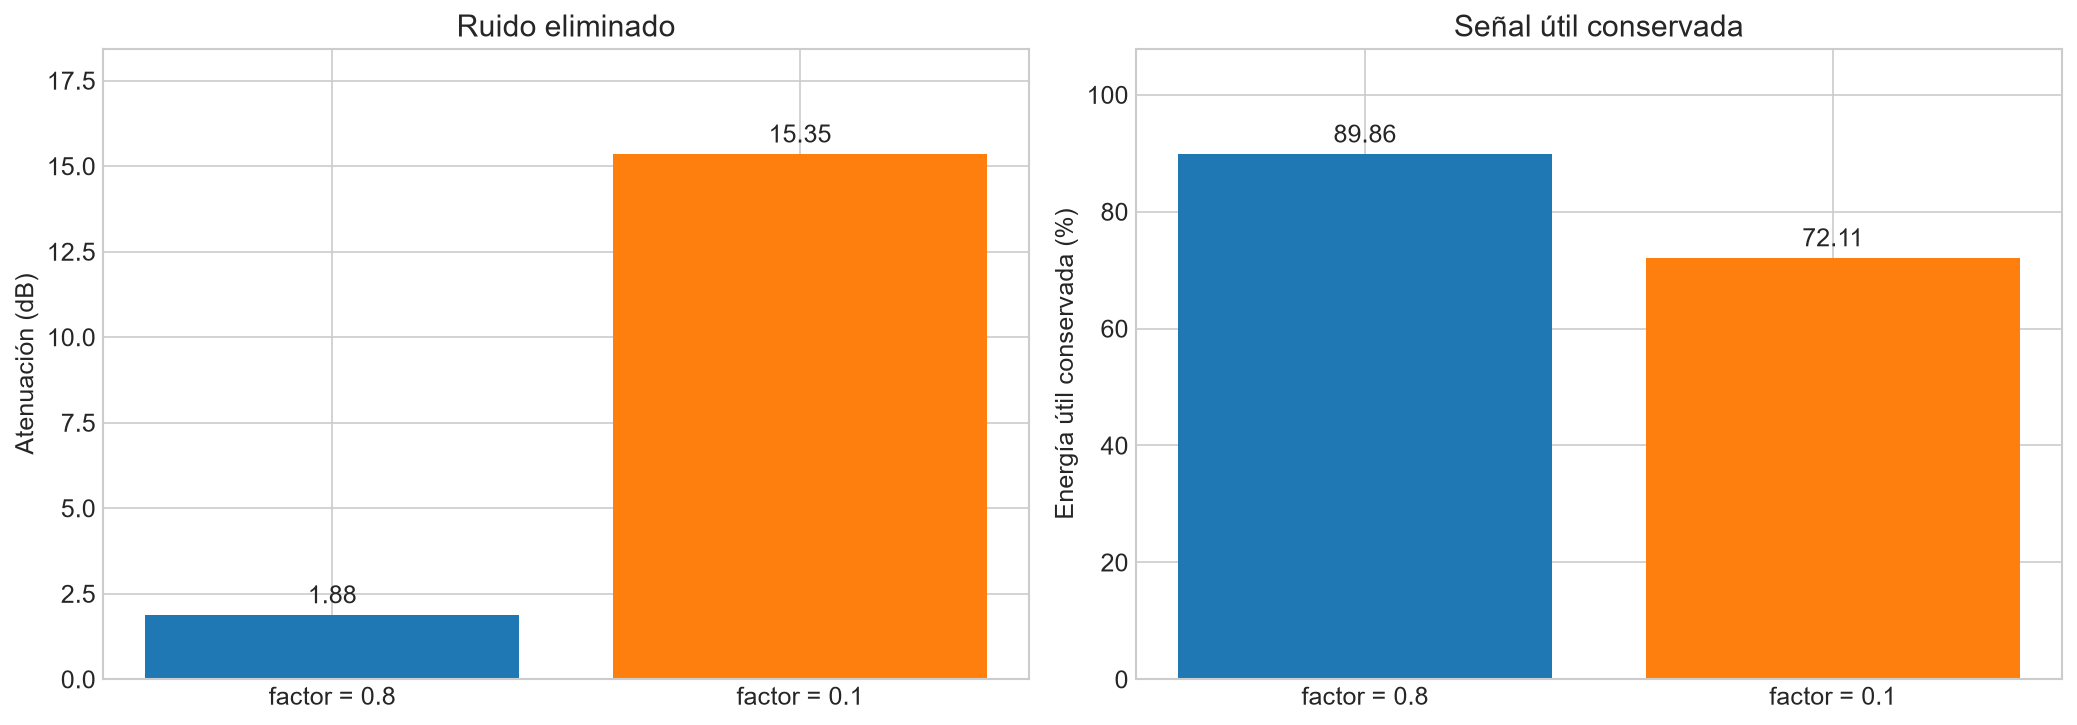
\includegraphics[width=0.85\linewidth]{espectral_compromiso_ruido_distorsion}
\caption{P5 con $f_{min}=600$ Hz: más supresión implica menos energía útil conservada.}
\label{fig:compromiso}
\end{figure}

\begin{figure}[H]
\centering
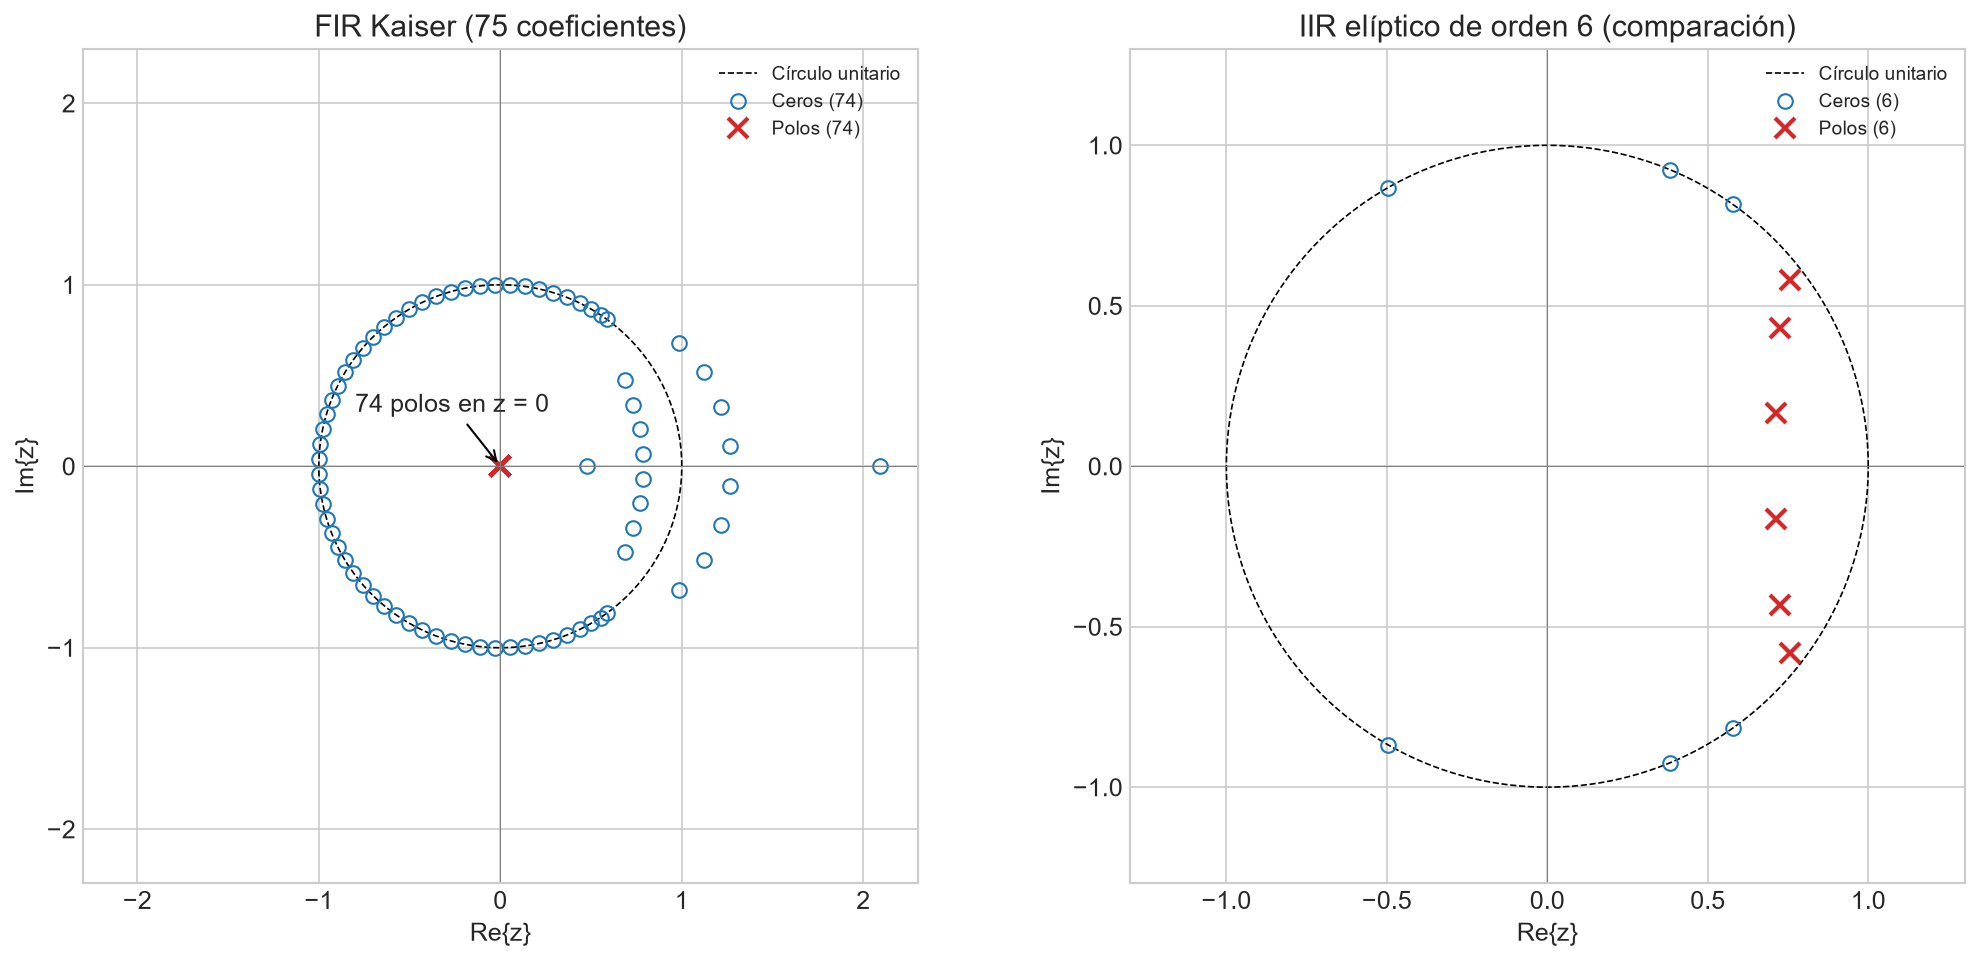
\includegraphics[height=2.6cm,clip,trim={0 0 475bp 0}]{fir_polos_ceros}\hspace{1mm}
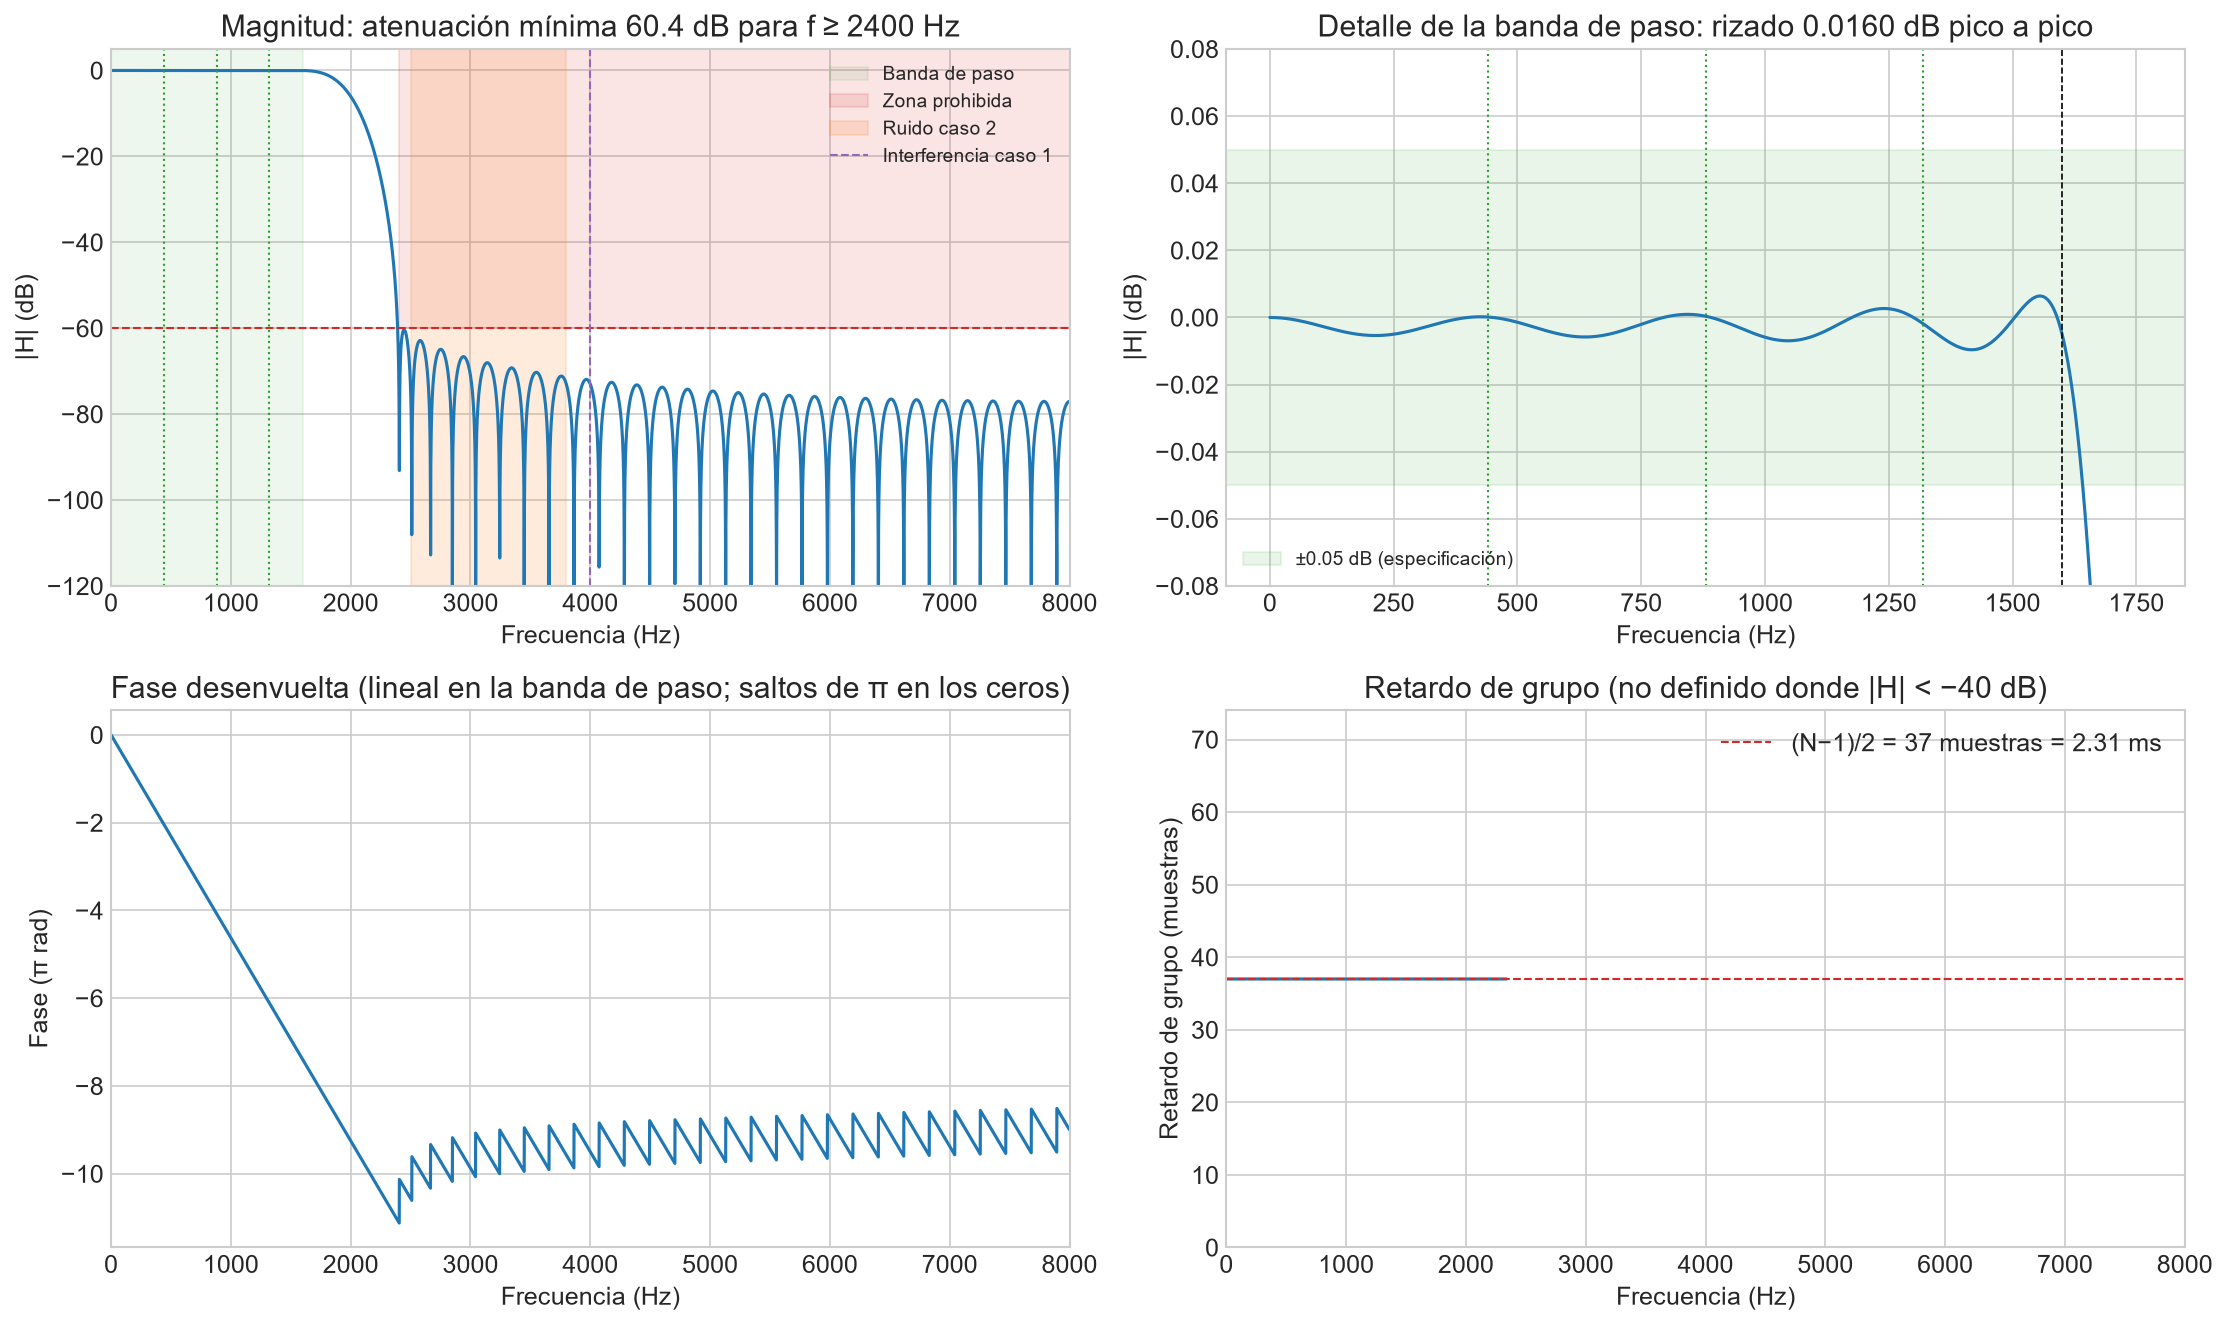
\includegraphics[height=2.6cm,clip,trim={0 318bp 534bp 0}]{fir_respuesta_frecuencia}
\caption{FIR Kaiser: polos y ceros; magnitud con rechazo $\geq60$~dB desde 2.4~kHz. Fase, retardo, IIR, FIR medido y respuesta analógica en las \href{\repo/docs/final/evidencias/README.md}{evidencias del repositorio}.}
\label{fig:fir}
\end{figure}




\end{document}
